\section{Preservation}
Currently, more and more information is produced in digital form and more and more information has only a digital copy. This has enourmous implications for national and state archives, libraries, scientific institutions and business enterprieses but also the small companies and even private people as they often face data corruption and access problems in the long-term.
In general, digital preservation (or DP for short) copes with two main problems; preserving content (bit streams) for longer periods of time and ensuring these contents are accessible and understandable in the future. When talking about ``the future'' or ``longer periods of time'' we mean ``as long the content is needed''.
Of course this view is over simplified and there are many more challenges in digital preservation. From the fundamental technical problems through organizational and social challenges to practical and financial ones.

A good example to picture the problem and challenges in DP is presented in \cite{Lorie:2001:LTP:379437.379726} and in \cite{Rauber:2009:dpchallenges}. Imagine a file created today on a specific physical machine. This file is nothing more than a series of bits shaped in a specific format. In order to access this file in the long term, not only the bits and bytes have to be preserved but also the way of interpreting them (the format specification). This would also require to preserve the programms that can open, render and manipulate the file, which in turn will require the preservation of the dependency libraries and software packages as well as the operating system and the whole environment in which these programms or programm versions run. Failing to preserve only one single part of this chain and the file would be lost (even if the physical bit stream is still in tact).

Due to this and many other problems a community of preservation experts has emerged. Through the last decade a number of DP-related research projects have been conducted that have identified problems and treats and have advanced the state of the art in this filed. An overview of the EU DP projects and activities is presented in this report \cite{strodl:2011:dpreport}. Starting in the mid nineties scientists recognized that these problems could lead to disasters and thus the need of digital preservation and its importance. By the beginning of the new millenium there were the first initiatives and projects in the EU that started focusing on research topics related to DP aiming the establishment of a community, identification of target groups and transfer of expertise (ERPANET\footnote{http://www.erpanet.org/}, DELOS\footnote{http://www.delos.info/}, DPE\footnote{http://www.digitalpreservationeurope.eu/}). The first scientific research was focused on topics such as standards, system concepts, selection and appraisal policies and fromat identification. Afterwards more technical and practical approaches were undertaken to research the preservation of simple digital objects such as office documents and images (PLANETS\footnote{http://www.planets-project.eu}, CASPAR\footnote{http://www.casparpreserves.eu}). All this helped the establishment of a solid community and a body of expertise.

Present initiatives include more fundamental research that tries to focus on more complex and interactive objects than simple and documents and data structures. Projects such as LiWA\footnote{http://www.liwa-pro ject.eu} attempt to solve issues related to Web Archiving whereas projects such as TIMBUS\footnote{http://timbusproject.net} and WF4Ever\footnote{http://www.wf4ever-pro ject.org} focus on the preservation of business processes and scientific workflows.
Other projects such as SCAPE\footnote{http://scape-project.eu} build upon the solid framework established in the past and aim to improve the state of the art of DP by developning infrastructure and tools for scalable preservation actions and integrating them with automated policy based preservation planning and preservation watch systems and workflows.
%what does the future hold
\subsection{Most Common Approaches}
% the tools at hand, why are these important, trade offs
Through the years many tools and procedures were developed in order to preserve digital content. In the literature there are often different names for the same concepts. Here we present the most prominent ones. \newline

\textbf{Bit-Stream Preservation}
is the concept of copying the bits to a different medium with a different (physical) location. There are many different media, which can store digital data. Some are more stable than others, some are more popular than others. No matter on what type of medium you choose to store your data, CDs, DVDs, HardDrives, etc. it is not guaranteed that the data stream is safe. Through physical damage, bit rot or other disasters, there is a high chance that your digital storage media will fail to reproduce your bit stream. Thus on this lower level your only option would be to copy the streams to a different medium from time to time. This is strategy is often referred to as \textit{refreshing} \cite{Lee:2002:SOTADP}.

However, refreshing the data does not guarantee that it will be accessible in a later point in time as new media are also error prone. Therefore, approaches like LOCKSS (Lots Of Copies Keep Stuff Safe) make use of the distribution of many independent copies. Developed at the Stanford University the LOCKSS approach was implemented in a librarian software system that deploys many low cost copies of persistent web-caches and enables the detection and repairment of damages based on voting in opinion polls \cite{reich2001lpw, Maniatis:2003:PPR:1165389.945451}.
%eventually say other projects that use LOCKSS (ExLibris, JISC, Hoppla, etc.)
Following a LOCKSS approach, however, only minimizes the risk of losing data. If there is no effort spent in management of the copies, then it is fairly easy to lose track of the copies. For a software tool this might seem irrelevant but for a private user this is a real issue. Furthermore, even if enough well-managed copies were stored and the data stream was preserved, there is always the issue of software obscolescense and thus failure in the access and interpretation of the stream. \newline

\textbf{Logical Preservation} tries to cope exactly with this problem. In order to preserve not only the bit stream but also to ensure that the integrity of a digital object and that it can be interpreted in the long-term a conversion or migration approach is used \cite{Lee:2002:SOTADP}. New operating systems, new software tools or new versions are sometimes incompatible or unable to render and manipulate older formats. To cope with technology changes digital preservation often uses a conversion strategy where the data is migrated to another format, that is usually considered to be more stable. Usually a format is considered worthy and stable for preservation purposes, when it is standardized, the format specification is open and well-documented, there are no patent owners and license fees that apply. The Florida Center for Library Automation for example offers a report\footnote{http://fclaweb.fcla.edu/uploads/recFormats.pdf} with the recommended data formats for preservation purposes that is considered as a good reference and starting point. However, there is no ultimate reference table or no ultimate file format that fits all preservation purposes. From use case to use case different aspects have to be considered. Neither standards, nor migration tools alone can ensure that a digital document remains accessible and its integrity remains unharmed. Rothenberg gives a good overview of common flaws of these concepts in \cite{rothenberg:1999:ensuring} and summarizes important aspects that should be considered in DP.

Nonetheless, logical preservation is often applied within digital preservation systems and repositories. As it also has potential pitfalls, it is not to be taken lightly.
Another more practical downside to migration are the storage costs. Often the target format has a bigger footprint than the original. Also the conversion of huge amounts of data is an error prone process that is not easy to validate \cite{Lorie:2001:LTP:379437.379726}. Furthermore, if the migration path consists of several steps one have to make sure that all required meta data of the original is also migrated to the new versions of the objects. Another related issue is also quality assurance. As it is infeasible to check manually if the conversion process was successful there are very specific requirements and processes that have to be followed in order to automate the verification of the preservation action \cite{feng:2010:qrofm}.
All these and other issues have to be carefully taken into account before choosing such a preservation action.
\newline

\textbf{Emulation} has the verb 'emulate' in its root, which means to immitate or reproduce.
In software terms an emulator is a software tool that immitates the behaviour of a (hardware) system/framework (usually an older one) in order to run other (obscolete) tools that are meant to run on the emulated system. Obviously, this approach offers can come in handy in regard of DP.
In \cite{rothenberg:1999:ensuring} Rothenberg gives an overview of a process for preservation that is based on an emulation process. The author states that not only the data (bit-stream) has to be stored but also the bit stream of the original program, the operating system and all other necessary parts, e.g. dependencies and used libraries. Also a thorough and complete description and specification of the underlying architecture have to be provided in a form that is readable by potential future emulator authors. If these prerequisites are met, an emulator that mimics the specific hardware needed to run the tool can be created.
Lorie points out in \cite{Lorie:2001:LTP:379437.379726} that the specification of the architecture has to be perfect and complete, which is a immensely difficult task. Another very important argument he makes is the evaluation of such an emulator. Even if all needed input exists and a hypothetical emulator was created, how can its correctnes as no original hardware device exists.

These and other reasons combined form one of the biggest downsides of emulation; cost. The effort, manpower and infrastructure needed to emulate an environment that renders digital documents is often more expensive than the value of the content of the documents themselves.

Nevertheless, emulation is widely used in specific branches, such as video gaming.
Guttenbrunner et al have evaluated different strategies for the preservation of console video games in \cite{guttenbrunner:2008:evaluating} and came to the conclusion that while migration shows very good results for the preservation of visual and audio components it completely fails in interactivity. Emulation on the other hand showed promissing results. All of these however, were strongly dependent on the sample objects that were emulated.

\subsection{Preservation Planning}
Preservation planning is a key task in DP that has to be undertaken by every institution or person that is serious about preservation. Numerous DP related projects have investigated the key requirements and processes involved in preservation planning. Projects such as PLANETS\footnote{http://www.planets-project.eu/} have created very strong fundaments in this area and have developed tools such as PLATO\footnote{http://ifs.tuwien.ac.at/dp/plato} - the preservation planning tool, which support the full planning workflow. Follow up projects, such as SCAPE\footnote{http://www.scape-project.eu/} advance the state of the art and enhance the planning capabilities by improving the current status, by building up a framework around the process that supports many new features such as preservation monitoring services and by automating the whole process in order to provide a scalable, robust preservation planning process.\newline

\noindent\textit{What is Preservation Planning?}\newline
The OAIS reference model was developed by the Consultative Committee for Space Data Systems and soon afterwards was dubbed to be an ISO standard \cite{iso:2003:oais}. This high-level reference model has proven to be a helpful tool for the DP community for many years. Undoubtedly, one of its key parts is preservation planning.

It is a decision making process that evaluates different preservation strategies or actions and chooses the most appropriate one. This process is highly dependent on object characteristics and institutional settings and requirements \cite{STR07_jcdl}. The goal of the process is to create a preservation plan that documents all the steps and choices that were made, the policies that were followed while making these decisions and the different preservation alternatives that were evaluated. It offers a complete documentation of the decision that allows one to repeat all experiments and verify why a certain preservation action was chosen.

The preservation plan is a very concrete artifact, opposed to policy documents, that specifies an action plan for the preservation of a set of digital objects.
\begin{quote}
A preservation plan defines a series of preservation actions to be taken by a responsible institution due to an identified risk for a given set of digital objects or records (called collection). The Preservation Plan takes into account the preservation policies, legal obli- gations, organisational and technical constraints, user requirements and preservation goals and describes the preservation context, the evaluated preservation strate- gies and the resulting decision for one strategy, includ- ing the reasoning for the decision. It also specifies a series of steps or actions (called preservation action plan) along with responsibilities and rules and condi- tions for execution on the collection. Provided that the actions and their deployment as well as the technical environment allow it, this action plan is an executable workflow definition \cite{Becker:2009fk}.
\end{quote}

PLATO\footnote{http://ifs.tuwien.ac.at/dp/plato} is a online tool developed at the University of Technology in Vienna, which supports the whole preservation planning workflow.
It guides the user through all necessary steps to create a fully documented (and executable) preservation plan. The workflow follows a process specific to a preservation planning environment as the one in figure \ref{fig:planenv}. The process constitutes from four main phases: define requirements, evaluate alternatives, analyze results and build preservation plan, all of which are covered by PLATO w.r.t the context of the current use case, such as the objects, the current technology, policies, etc.
There is also an external monitoring phase which feeds back important information about relevant changes in the environment, which can cause a reiteration/reevaluation of a preservation plan. A detailed overview and a high level design of such an addition to the preservation planning enviroment can be found in \cite{duretec:2012:watch}.

\begin{figure}[tbh]
\begin{center}
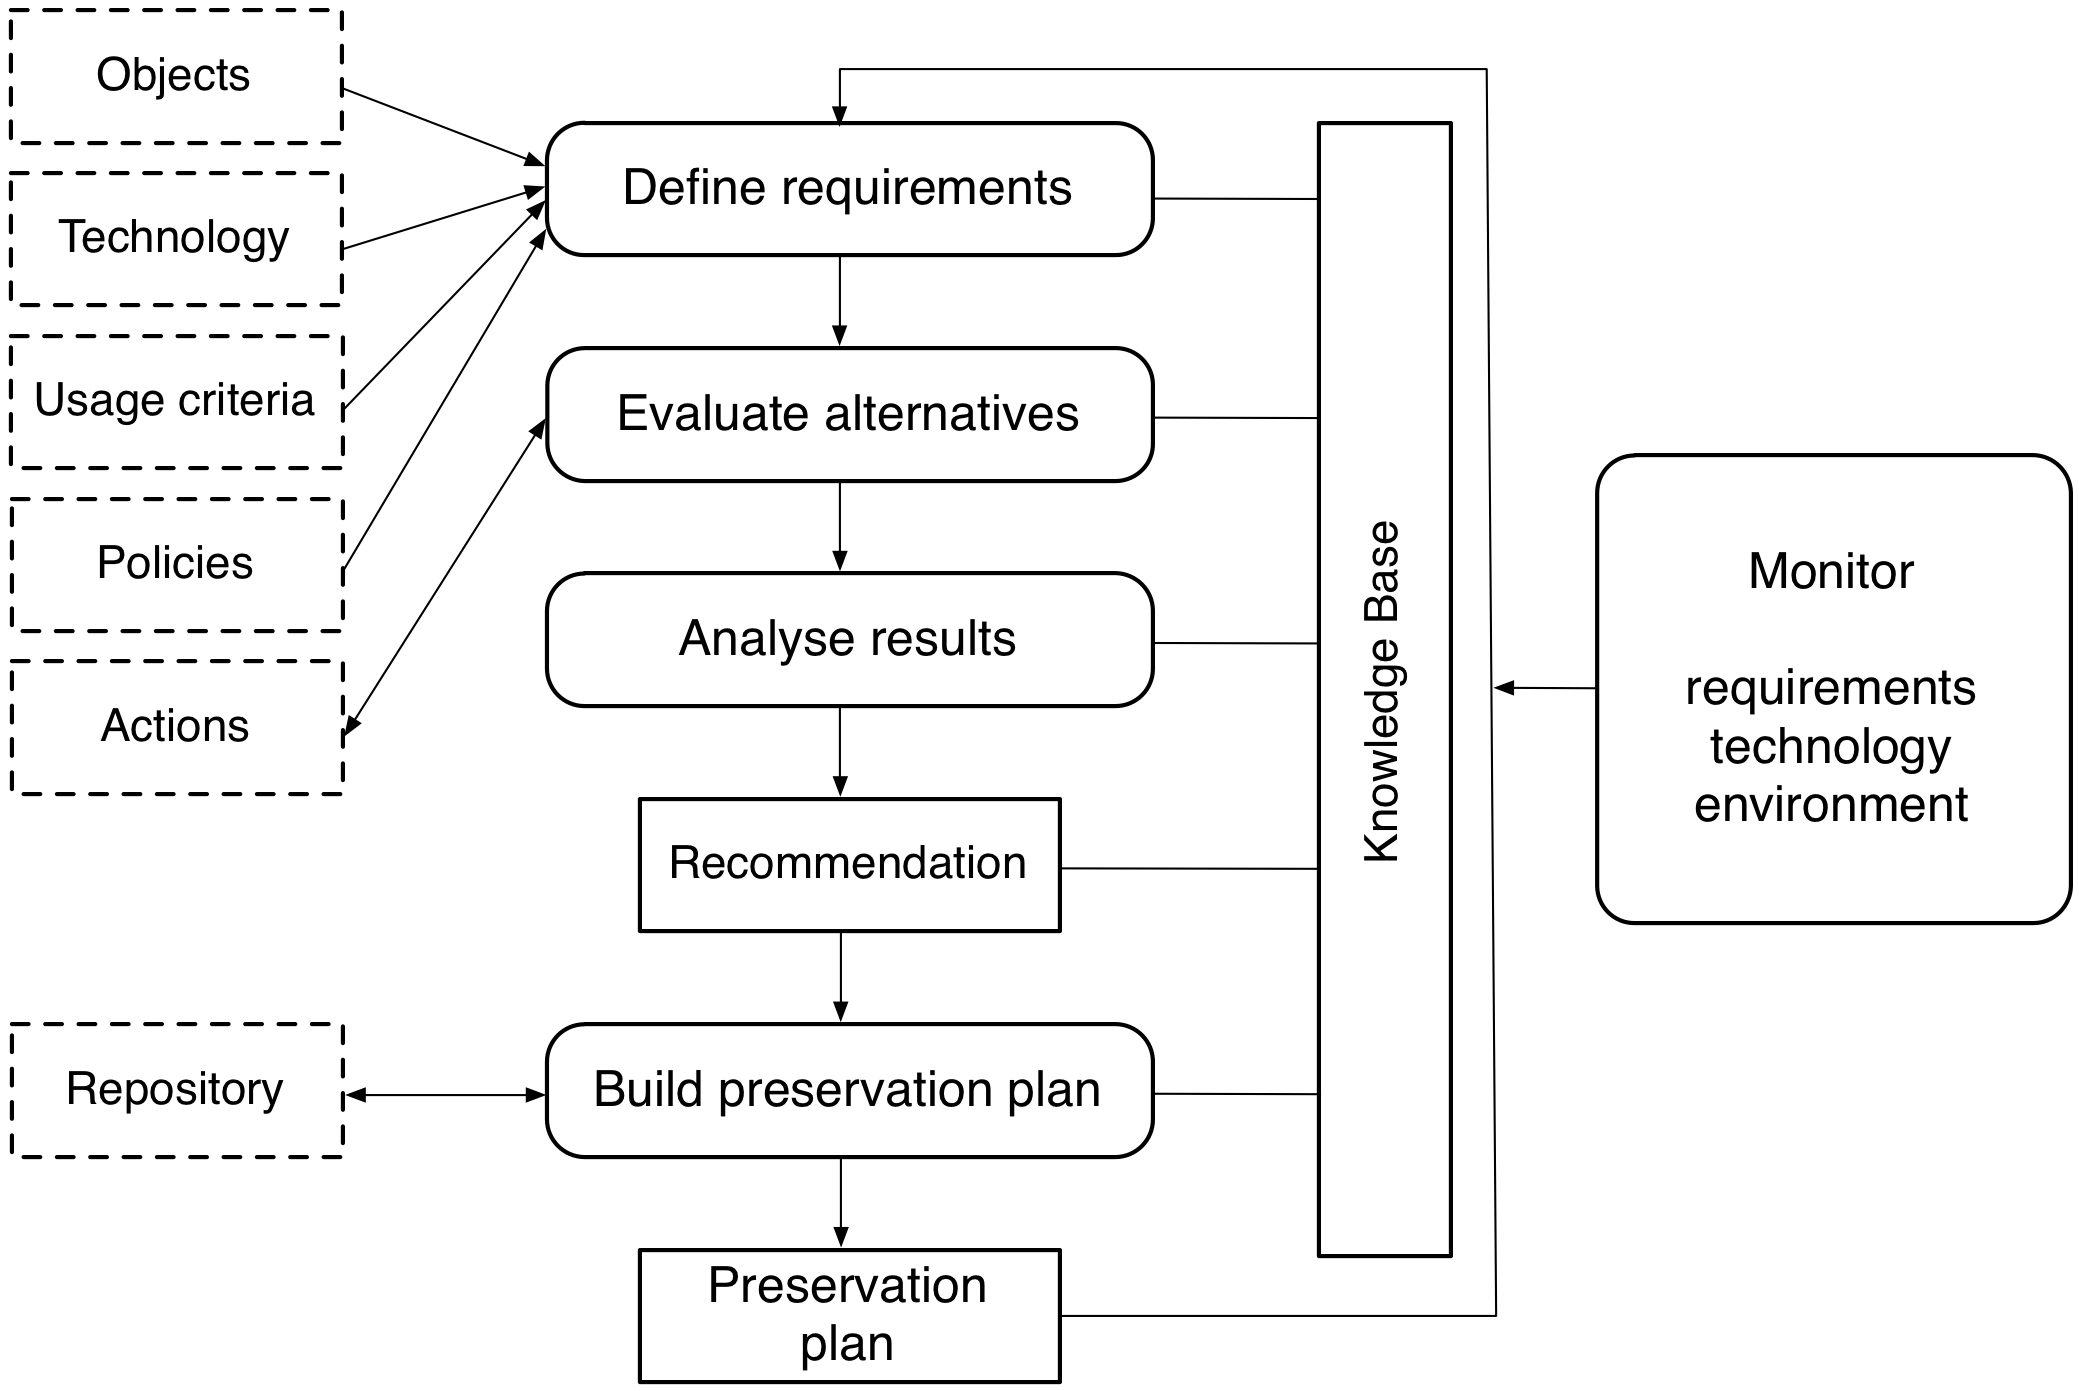
\includegraphics[width=5in]{figures/related/planningenvironment.png}
\caption{The preservation planning environment \cite{becker:2010:trustowrothy}.}
\label{fig:planenv}
\end{center}
\end{figure}

%A key aspect of a preservation plan is the description of the collection. It includes general characteristics and allows the stratification of sample objects, which are the basis for the experiments and evaluation of the potential preservation actions.


%what it is, overview, steps, Plato, etc.
% the big picture
\section{Analyzing Collections}
A collection here is defined as a set of digital objects that was created by some process or a user for some specific reason. Whether all digital objects are stored on the same physical location, how they are managed is irrelevant in this context. It is important to keep in mind that a set of digital objects exists and all of its objects are related for some reason.

Obviously, to create and analyze such a collection the meta data for each object has to be examined. Meta data is a descriptive information, usually stored within a file, that provides further information about the content and format of the file.

Furthermore, analysis of such a huge content often is done in a manual fashion, which can be a very time-consuming and cumbersome task. It is obvious if there would be tools at hand, such as identification and characterization, data aggregation, filtering, collection splitting, etc., which will automate the process to a certain degree, that this task will be handled much faster and potentially much more efficient. \newline

\textbf{Identification vs. Characterization}

Based on different properties/characteristics a collection can be dubbed homogeneous or heterogeneous. Usually to a user a homogeneous collection would be a set of files that consists only or mostly of objects having the same format or even the same type (audio, video, text, etc.). This however, is an oversimplification, which has enourmous side effects for preservation planning.

Consider the following example where a collection consists of N digital objects, which share the same extension, e.g. 'pdf'. To a normal user this would be a homogeneous collection. An advanced user, however, would know that the extension of a file does not really specify the format of the file and thus could assume that there are differences.
One step further would be to conduct an identification process that looks for the specific file format and format version. Assume that in our example 95\% of all files have the same pdf format and format version.  Then this could be considered a homogeneous collection w.r.t to format. 
In a next step, however, characterization is conducted and now there are many more properties, such as \textit{creating applicatons}, \textit{encryption}, \textit{password protection}, \textit{tags}, etc.
Regarding these characteristics the same collection can be considered to be heterogeneous.
Obviously, all of this is very important to preservation planning, since different preservation actions produce different results exactly because of such differences.

Thus the question remains, how to identify such important properties that define the homgenity of a collection? Following this train of thought, obviously the format is a very important characteristic, however, it does not cover all cases (as in the example) and many others are important. \newline

% what is important here
% what is identification, what is characterization.
% meta data, distributions, aggregations, scalability, etc.
% homgeneous vs heterogeneous collections
% some properties are obviously more important than others.
% is the format ultimate significant property...

\textbf{Statistical Data and Aggregation}

As collections in DP are often just too large for a human being to comprehend, obviously the meta data provided by identification and characterization has to be aggregated in some fashion. Furthermore, different statistical information will ease the understanding and stratification of the content into different homogeneous parts. Often simple statistics, such as min, max, avg, sd, etc. provide meaningul information about the current content one has to deal with. Moreover, histogramms and distributions of mimetypes, formats, format version and other properties help to create the bigger picture of the content that is to be preserved. \newline

\textbf{Filtering, Splitting and Representatives}

Once the bigger picture gets clearer the collection can be divided into different (more) homogeneous parts, which will ease the decisions that have to be made regarding their future with respect to DP and PP.
Another important part would be finding representative sets within the homogeneous content, which forms a better suited common ground for the experimentation phase of the preservation planning process. Finding these small subsets within homogeneous collections is potentially much easier than in heterogeneous context. This problem will be furtherly investigated in later parts of this thesis.

\section{Tools and Meta Data}
There are numerous software projects and tools that are related to DP and focus on the field of identification and characterization. In this section we observe some of the most prominent ones. A recent report (created as part of the SCAPE project) summarizes an evaluation framework and the results of the tests of several identification and characterization tools \cite{Knijff:2011it}. It provides a rather good overview of the current state of the art of such tools but concentrates mostly on their identification capabilities. In the report six tools (DROID 6.0, Fido 0.9, Unix File Tool, FITS 0.5 and JHOVE2) were evaluated against 22 criteria among which, the tool interface, its license type, platform dependencies, accuracy of reported results, documentation, etc.

Here we summarize the strengths and weaknesses of these and some other tools briefly.

\begin{itemize}
\item \textbf{DROID 6.0}\newline
Droid is an identification tool produced by the National Archives, which uses the PRONOM\footnote{www.nationalarchives.gov.uk/pronom/} registry and its format signatures and/or file extensions. It provides information about the mimetype, format and format version of a file as long it is in the DROID signature file, which contains the 'magic numbers' of the PRONOM registry. It also outputs a PRONOM Unique Identifier or puid, which can be used to trace the format back into the registry.
Unfortunately, the registry is not open and its maintanence is slow. However, the tool is very useful and widely used within the DP community.

\item \textbf{Apache TIKA}\newline
Tika is an open source project from The Apache Software Foundation that is able to extract metadata from files with various formats. It is a stable tool able to identify files by analysing their bitstream and allows the deeper characterization of some of these files.  

\item \textbf{FIDO 0.9}\newline

\item \textbf{UNIX File Tool}\newline

\item \textbf{FITS} \newline
The File Information Tool Set is developed by the Harvard University Library. It wraps common identification and characterization tools as the ones described here and tries to consolidate them and provide a normalized output. By providing basic provenance information for each extracted record it combines the consolidation result and provides a very basic confidence status for the extracted value of each property. This prooves to be helpful for cases where there are uncertainties. The framework is designed to be extended, so that other tools can be also added. The tool seems very helpful, although there are some unstabilities and problematic cases.

\item \textbf{JHOVE}\newline
JHOVE is one of the most well-known identification and characterization tools used by the DP community. It is also developed by the Harvard University Library and is able to extract meta data from various formats based on different modules. Probably one of the most valuable features of JHOVE is the ability the check a file for wellformedness and validity against the format specification.

\item \textbf{JHOVE 2}\newline
JHOVE 2 is a successor project for the JHOVE tool and also provides an extensible architecture for characterization tools and modules. It is developed as an open source tool by the California Digital Library, Portico and Stanford Univeristy. Currently it produces helpful output only for a few types of documents as the different modules are not yet developed.

\end{itemize}

Although this list is not complete, and there are many other tools that are able to extract meta data as well it shows that the current state of the art is able to provide enough meta data that could be used as input for various preservation activities. The tools have their downsides in terms of format coverage and/or performance, but still provide very valuable information.
Currently there are only a few tools however, that are able to analyze collections. PRONOM ROAR, for example, is able to create a format profile within a repository interface with the help of DROID.
Various repositories provide basic information as the formats and size of objects, however no further stratification is possible, although the characterization data is present.

% what is present.
% explain that the tools for different types of contents are there, but no tool does
% collection profiling
% scape evaluation of characterisation...


\section{Quality Assurance}
One of the biggest downsides of all identification and characterization tools is the lack of quality assurance processes. Often there is no way to validate if an extracted measurement value is really representing the truth. This is a huge problem, as it is hard to make assumptions about validity without having a ground truth.
Some tools such as FITS try to tackle this problem on a very basic level by stating a confidence level in the form of an enumeration (OK, SINGLE\_RESULT, PARTIAL, CONFLICT). It is not perfect, but it provides the user with warnings about potential treats.
A big problem here is the consolidation. Often tools provide the same measurement for a specific property but the output format is different. This makes it hard for an automatic consolidator to decide if the values are equal or not. Thus the problem of quality assurance depends on external information provided by other processes or even by manual verification. 
Obviously, this is a hard, tedious and long running process and thus it is (partially) neglected.
Nonetheless, it is an essential precondition in order to assure correct input data for the analysis.
% despite the tools there is a big gap
% tools extract some measures, but there is almost no way, to assure that
% a measurement is correct
% often tools extract the same information and represent it in different way, thus providing a conflict - verification is hard...
% JHove validation, verification

\section{Observations}
In order to prepare a preservation action plan some prerequisites have to be met. The following provides a simplified list of steps that would occur in a common digital preservation scenario, usually in the following order: 
\begin{enumerate}
\item Organizational policies about the management of the content are created and curated.
\item As part of the repository ingest an identification and deep characterization process extracts valuable meta data and stores it within the repository.
\item A content profile is generated and exported for other tools.
\item A monitoring component identifies that a certain subset of objects violates the policies and notifies a planning expert for the potential treat.
\item A planner uses the content profile, a profiler to analyse and stratify the content into smaller homogeneous partitions as well as identify representative sample objects for the partitions.
\item A planning tool is used to validate the treat and to create an action plan that is able to cope with the policy violations.
\item The action plan is submitted to a repository, which knows how to execute the described preservation action.
\item The monitoring component observes the operations of the repository and notifies the interested parties of important events, such as throughput, failures and task executions. 
\item The violation is taken care of and the monitor component continues its work.
\end{enumerate}

The state of the art provides some of these components and actors in this high-level workflow. Any organization, which is serious about digital preservation has its own set of policies of how to handle different types of content. The problem here is that often such policies are just high-level descriptive statements, which are not structured in any specific form and thus are not machine readable. This makes it almost impossible to use in automated fashion. Also there are numerous repositories that can manage digital objects and extract meta data from them. The planning tool Plato provides the needed facilities to create an action plan.

However, a couple of components are missing. A preservation monitor, that scans relevant properties of the world and evaluates their values for changes, eventually notifying users or other agents of interesting events. Such a monitor is currently developed within the SCAPE Project (TODO cite).
Another crucial part that is missing is a tool able to profile a massive content set and stratify it into smaller homogeneous and managable partitions. If there was such a tool it would provide two main benefits. First, easier analysis and content stratification and thus better foundation for planning experiments with reduced bias and second input to a preservation monitor that will be able to create a global profile of content, which would be of great benefit to the DP community.

% summarize, what is going on,
% what is missing
% what is the problem of the current state of the art
% based on the research you made.